\section{DC Sweep Simulation}
The schematic in the first exersice with \textbf{R1 = 1k} is re-used in this exercise. However, a DC-Sweep simulation mode is performed with V1 is varied from 0V to 5V (0.1V for the step), as follows:

\begin{figure}[!htp]
    \centering
    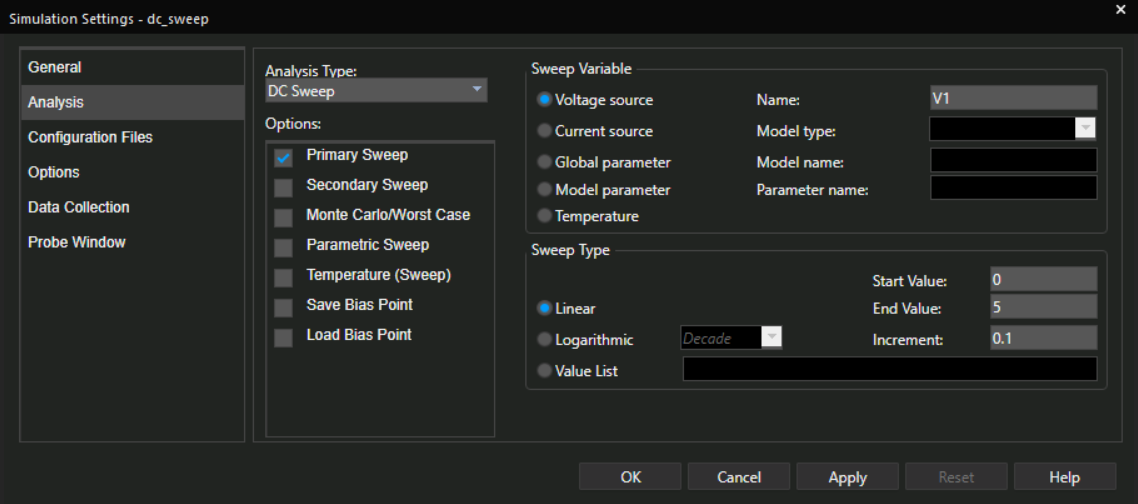
\includegraphics[width=4in]{graphics/ex2/f1.PNG}
    \caption{\textit{DC-Sweep profile for simulation}}
    % \label{bai3_manual_2}
\end{figure}

Run the simulation and trace for the current $I_C$ according to the value of V1. Capture your screen and plot it in the report. Please increase the width of the curve.